\documentclass[presentation]{beamer}
\mode<presentation>{\usetheme{AMSBolognaFCrev}}

\usepackage[utf8]{inputenc}
\usepackage[T1]{fontenc}
\usepackage{booktabs}
\usepackage{array}
\usepackage{colortbl}
\usepackage{tikz}
\usepackage[ddmmyyyy]{datetime}
\usepackage[export]{adjustbox}
\usetikzlibrary{arrows.meta,positioning,shapes.geometric}

\renewcommand{\dateseparator}{/}
\newcommand{\sectiontitleframe}[1]{
\begin{frame}[plain,c]
\begin{center}
{\usebeamerfont{title}\usebeamercolor[fg]{title}#1}
\end{center}
\end{frame}
}

\title[Lesson 1]{Foundations of Computer Security in Healthcare}
\institute[Data Privacy and Security]{Healthcare Data Privacy and Security}
\author[\sspeaker{G. Pisano}]{\speaker{Giuseppe Pisano} \\\href{mailto:g.pisano@unibo.it}{g.pisano@unibo.it}}
\date[August, 2026]{August, 2026}
%
\titlegraphic{
%\vspace{0.2cm}
\begin{center}
    
\includegraphics[width=0.35\textwidth, valign=c]{logos/intestazione.png}
    
\includegraphics[width=0.16\textwidth, valign=c]{logos/unibo_logo_2.png}
    
\includegraphics[width=0.11\textwidth, valign=c]{logos/makeni_logo_2.png}
    
\includegraphics[width=0.20\textwidth, valign=c]{logos/cuamm_logo_png.png}
\end{center}
\centering
\tiny{S.K.I.L.L.E.D --- AID013244/04/2\\Strategic Knowledge and Inclusive Lifelong Learning in the health sector for youth Employability and Development}
}

\begin{document}

\setbeamertemplate{frametitle}
{
    \nointerlineskip
    \begin{beamercolorbox}[sep=0.3cm,ht=2.2em,wd=\paperwidth]{frametitle}
        \vbox{}\vskip-2ex%
        \strut\insertframetitle\hfill\raisebox{-0.2\height}{
\includegraphics[width=2cm]{logos/cuamm_logo_png.png}}\strut
        \vskip-0.8ex%
    \end{beamercolorbox}
}

\begin{frame}[allowframebreaks]
\titlepage
\end{frame}

\begin{frame}[c,allowframebreaks]{Roadmap}
\tableofcontents[hideallsubsections]
\end{frame}


\begin{frame}[c]{How This Lesson Progresses}
\begin{block}{Learning path}
We will move from \textbf{what must be protected}, to \textbf{where it lives}, to \textbf{how it can fail},
and finally to \textbf{how security choices reduce risk}.
\end{block}

\begin{exampleblock}{Hospital storyline}
St. Isidore Hospital gives us one continuous scenario: first we identify the systems and security
objectives, then we examine risks and attacks, and finally we discuss how design and policy shape
safer clinical workflows.
\end{exampleblock}
\end{frame}

\begin{frame}[c]{From This Lesson to the Next Topics}
\begin{block}{Why the order matters}
The concepts in this lesson are the vocabulary for the rest of the course. Later lessons will go
much deeper into the technical, organisational, and legal controls.
\end{block}

\begin{itemize}
    \item \textbf{Basic networking}: explains the hospital communication paths we identify today.
    \item \textbf{Access management}: turns confidentiality, authenticity, and accountability into roles and permissions.
    \item \textbf{Encryption}: protects confidentiality and integrity in storage and transmission.
    \item \textbf{GDPR}: frames security as part of lawful, fair, accountable processing of personal data.
\end{itemize}
\end{frame}

\section{Running Scenario}
\sectiontitleframe{Running Scenario}

\begin{frame}[c]{Section Context: Running Scenario}
\begin{block}{What we are talking about}
Before introducing formal security concepts, we establish a shared hospital environment. This
keeps the lesson practical: every definition will be connected to a concrete clinical workflow,
system, user, or failure mode.
\end{block}

\begin{exampleblock}{Why it matters}
In healthcare, security decisions are never abstract. A control that looks reasonable on paper can
affect triage, medication delivery, lab turnaround time, or patient trust.
\end{exampleblock}
\end{frame}

\begin{frame}[c]{The Hospital We Will Use}
\begin{block}{Running example: St. Isidore Hospital}
St. Isidore is a mid-size hospital with an emergency department, wards, a laboratory,
radiology, pharmacy, billing office, and a small IT team.
\end{block}

\begin{exampleblock}{Digital systems}
The hospital uses an \textbf{EHR}, a \textbf{laboratory system}, a \textbf{PACS} for medical images,
a \textbf{pharmacy system}, staff laptops, Wi-Fi, remote access for doctors, and a few connected
medical devices.
\end{exampleblock}
\end{frame}

\begin{frame}[c]{Scheme: Hospital Digital Ecosystem}
\begin{center}
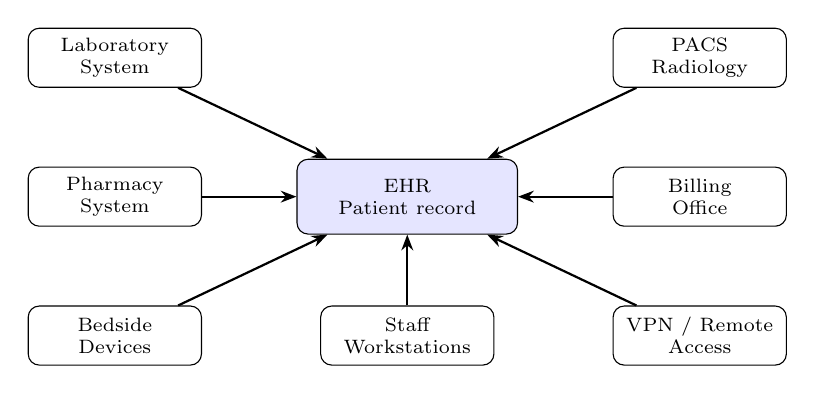
\begin{tikzpicture}[
    node distance=0.9cm and 1.2cm,
    system/.style={draw, rounded corners, align=center, minimum width=2.2cm, minimum height=0.75cm, font=\scriptsize},
    core/.style={system, fill=blue!10, minimum width=2.8cm, minimum height=0.95cm},
    link/.style={-{Stealth[length=2mm]}, thick}
]
\node[core] (ehr) {EHR\\Patient record};
\node[system, above left=of ehr] (lab) {Laboratory\\System};
\node[system, above right=of ehr] (pacs) {PACS\\Radiology};
\node[system, left=of ehr] (pharm) {Pharmacy\\System};
\node[system, right=of ehr] (billing) {Billing\\Office};
\node[system, below left=of ehr] (devices) {Bedside\\Devices};
\node[system, below=of ehr] (staff) {Staff\\Workstations};
\node[system, below right=of ehr] (remote) {VPN / Remote\\Access};
\draw[link] (lab) -- (ehr);
\draw[link] (pacs) -- (ehr);
\draw[link] (pharm) -- (ehr);
\draw[link] (billing) -- (ehr);
\draw[link] (devices) -- (ehr);
\draw[link] (staff) -- (ehr);
\draw[link] (remote) -- (ehr);
\end{tikzpicture}
\end{center}

\begin{block}{Reading the scheme}
The EHR is central, but security depends on every connected system, user, and network path.
\end{block}
\end{frame}

\begin{frame}[c]{Why This Scenario Matters}
\begin{block}{Key idea}
Security in healthcare is not only about protecting computers. It protects \textbf{patients},
\textbf{clinical decisions}, \textbf{care continuity}, and \textbf{trust}.
\end{block}

\begin{exampleblock}{Hospital example}
If the EHR is unavailable during a night shift, clinicians may not see allergies, medications, or
recent lab results. A technical failure becomes a \textit{patient-safety} issue.
\end{exampleblock}
\end{frame}

\begin{frame}[c]{Recap: Running Scenario}
\begin{block}{Takeaways}
\begin{itemize}
    \item We will use \textbf{St. Isidore Hospital} as the running example throughout the lesson.
    \item The hospital combines clinical systems, administrative systems, networks, devices, and people.
    \item Security protects \textit{care delivery}, not only servers and databases.
\end{itemize}
\end{block}
\end{frame}

\section{Security Objectives}
\sectiontitleframe{Security Objectives}

\begin{frame}[c]{Section Context: Security Objectives}
\begin{block}{What we are talking about}
This section explains the goals security is trying to achieve. The key question is:
\textit{what does it mean for a hospital system to be secure?}
\end{block}

\begin{exampleblock}{Hospital lens}
For St. Isidore, a secure EHR is not merely hidden from outsiders. It must be readable by the
right clinicians, accurate enough to support care, available during work, and traceable when used.
\end{exampleblock}
\end{frame}

\begin{frame}[c]{Computer Security}
\begin{block}{Definition}
Computer security is the protection provided by an information system to preserve the security
objectives of the system and its resources. NIST frames the core objectives as
\textbf{confidentiality}, \textbf{integrity}, and \textbf{availability} \cite{nist_fips_199}.
\end{block}

\begin{exampleblock}{Hospital example}
St. Isidore must protect patient records, clinical software, network links, staff accounts,
medical images, backup systems, and devices used at the bedside.
\end{exampleblock}
\end{frame}

\begin{frame}[c]{System Resources}
\begin{block}{Concept}
A system resource is anything the organisation depends on to deliver information services.
\end{block}

\begin{itemize}
    \item \textbf{Hardware}: servers, laptops, scanners, network devices.
    \item \textbf{Software}: EHR, PACS, pharmacy and laboratory systems.
    \item \textbf{Data}: clinical notes, lab results, images, prescriptions.
    \item \textbf{Telecommunications}: Wi-Fi, VPN, internal network, Internet links.
\end{itemize}

\begin{exampleblock}{Hospital example}
An MRI image is data; the PACS is software; the storage server is hardware; the link between
radiology and the ward is telecommunications.
\end{exampleblock}
\end{frame}

\begin{frame}[c]{The CIA Triad}
\begin{block}{Core model}
The CIA triad summarises three central security goals:
\textbf{confidentiality}, \textbf{integrity}, and \textbf{availability}.
\end{block}

\begin{exampleblock}{Hospital example}
For a medication order, \textbf{confidentiality} means only authorised staff can see it;
\textbf{integrity} means the dose is not changed incorrectly; \textbf{availability} means the order is
reachable when the nurse administers treatment.
\end{exampleblock}
\end{frame}

\begin{frame}[c]{Scheme: CIA for a Medication Order}
\begin{center}
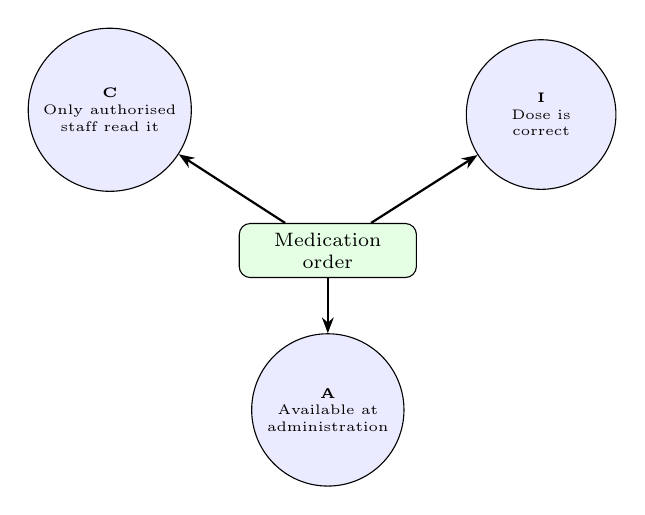
\begin{tikzpicture}[
    node distance=0.7cm and 0.9cm,
    goal/.style={draw, circle, align=center, minimum size=1.9cm, font=\tiny, fill=blue!8},
    asset/.style={draw, rounded corners, align=center, minimum width=2.25cm, minimum height=0.65cm, font=\scriptsize, fill=green!10},
    link/.style={-{Stealth[length=2mm]}, thick}
]
\node[asset] (order) {Medication\\order};
\node[goal, above left=of order] (c) {\textbf{C}\\Only authorised\\staff read it};
\node[goal, above right=of order] (i) {\textbf{I}\\Dose is\\correct};
\node[goal, below=of order] (a) {\textbf{A}\\Available at\\administration};
\draw[link] (order) -- (c);
\draw[link] (order) -- (i);
\draw[link] (order) -- (a);
\end{tikzpicture}
\end{center}

\smallskip
\centering
\textbf{Takeaway:} the same clinical object must satisfy all three goals at once.
\end{frame}

\begin{frame}[c]{Confidentiality}
\begin{block}{Concept}
\textbf{Confidentiality} means that information is accessed and disclosed only according to
authorised rules.
\end{block}

\begin{itemize}
    \item It is not secrecy from everyone.
    \item It is \textit{controlled disclosure} to the right people for the right purpose.
\end{itemize}

\begin{exampleblock}{Hospital example}
An emergency doctor may view a patient's allergies. A billing clerk may view insurance data.
Neither should automatically see psychotherapy notes unrelated to their role.
\end{exampleblock}
\end{frame}

\begin{frame}[c]{Privacy}
\begin{block}{Concept}
\textbf{Privacy} concerns how personal information is collected, stored, used, shared, and retained.
\end{block}

\begin{itemize}
    \item Confidentiality protects access to information.
    \item Privacy also asks whether the information should be processed at all.
\end{itemize}

\begin{exampleblock}{Hospital example}
A research team may need aggregated diabetes statistics. Privacy requires minimisation,
consent or another lawful basis, and removal of unnecessary identifiers.
\end{exampleblock}
\end{frame}

\begin{frame}[c]{Data Integrity}
\begin{block}{Concept}
\textbf{Data integrity} means that information is accurate, complete, and modified only through
authorised and expected processes.
\end{block}

\begin{exampleblock}{Hospital example}
If a patient's allergy to penicillin is deleted or changed, the record may still be confidential
and available, but it is no longer safe to trust.
\end{exampleblock}
\end{frame}

\begin{frame}[c]{System Integrity}
\begin{block}{Concept}
\textbf{System integrity} means that the system performs its intended functions without
unauthorised manipulation.
\end{block}

\begin{exampleblock}{Hospital example}
The pharmacy system should calculate interactions and dosage warnings according to approved
rules. If malware changes those rules, the system may give unsafe recommendations.
\end{exampleblock}
\end{frame}

\begin{frame}[c]{Availability}
\begin{block}{Concept}
\textbf{Availability} means that information and services are reachable when they are needed.
\end{block}

\begin{itemize}
    \item Outages matter.
    \item Severe slowness also matters.
    \item Missing dependencies can break a service even if the application itself is healthy.
\end{itemize}

\begin{exampleblock}{Hospital example}
If the EHR login service fails, clinicians cannot access records even if the EHR database is
still intact.
\end{exampleblock}
\end{frame}

\begin{frame}[c]{Authenticity}
\begin{block}{Concept}
\textbf{Authenticity} gives confidence that a user, device, message, or data source is genuine.
\end{block}

\begin{exampleblock}{Hospital example}
When the lab system sends a potassium result to the EHR, the EHR must know it really came from
the laboratory system, not from a forged message.
\end{exampleblock}
\end{frame}

\begin{frame}[c]{Accountability}
\begin{block}{Concept}
\textbf{Accountability} links actions to identifiable entities. It supports audit, investigation,
deterrence, and legal responsibility.
\end{block}

\begin{exampleblock}{Hospital example}
If a celebrity patient is admitted, audit logs should show which staff members opened the record,
when, and from which workstation.
\end{exampleblock}
\end{frame}

\begin{frame}[c]{Recap: Security Objectives}
\begin{block}{Takeaways}
\begin{itemize}
    \item \textbf{Confidentiality} controls who can see sensitive information.
    \item \textbf{Integrity} keeps data and system behaviour trustworthy.
    \item \textbf{Availability} keeps clinical services reachable when needed.
    \item \textbf{Authenticity} and \textbf{accountability} make actions reliable and traceable.
\end{itemize}
\end{block}

\begin{exampleblock}{Hospital checkpoint}
A medication order is secure only if it is seen by authorised staff, unchanged, available at
administration time, issued by a genuine clinician, and auditable afterwards.
\end{exampleblock}
\end{frame}

\section{Components and Networks}
\sectiontitleframe{Components and Networks}

\begin{frame}[c]{Section Context: Components and Networks}
\begin{block}{What we are talking about}
This section looks at where threats land in a real system: hardware, software, data, and
communication lines. Network security matters because hospital systems are connected by many
paths and dependencies.
\end{block}

\begin{exampleblock}{Hospital lens}
An EHR outage may start with a stolen laptop, a vulnerable application, corrupted data, or a
network attack. Understanding the component helps choose the right control.
\end{exampleblock}
\end{frame}

\begin{frame}[c]{Hardware Threats}
\begin{block}{Concept}
Hardware is especially exposed to physical threats: theft, damage, tampering, and loss.
\end{block}

\begin{exampleblock}{Hospital example}
A laptop containing cached patient data is stolen from a clinic room. Full-disk encryption and
remote wipe reduce confidentiality risk.
\end{exampleblock}
\end{frame}

\begin{frame}[c]{Software Threats}
\begin{block}{Concept}
Software can be deleted, copied, misconfigured, or modified so that it behaves differently from
what users expect.
\end{block}

\begin{exampleblock}{Hospital example}
A malicious browser extension on a workstation captures EHR session data. Application allowlisting
and endpoint monitoring help reduce this risk.
\end{exampleblock}
\end{frame}

\begin{frame}[c]{Data Threats}
\begin{block}{Concept}
Data must be protected for confidentiality, integrity, and availability at the same time.
\end{block}

\begin{exampleblock}{Hospital example}
Backups protect availability, access control protects confidentiality, and audit trails help
detect unauthorised modification of patient records.
\end{exampleblock}
\end{frame}

\begin{frame}[c]{Communication-Line Threats}
\begin{block}{Concept}
Network communication can be read, blocked, delayed, modified, duplicated, or reordered.
\end{block}

\begin{exampleblock}{Hospital example}
A lab result message delayed between the laboratory system and the EHR may cause clinicians to
act on outdated information.
\end{exampleblock}
\end{frame}

\begin{frame}[c]{Passive Network Attacks}
\begin{block}{Concept}
Passive network attacks observe communication without changing it. They are hard to detect
because systems continue to work normally.
\end{block}

\begin{exampleblock}{Hospital example}
Traffic analysis shows that a VIP patient's room communicates frequently with oncology and
radiology, revealing sensitive context without reading message contents.
\end{exampleblock}
\end{frame}

\begin{frame}[c]{Active Network Attacks}
\begin{block}{Concept}
Active network attacks modify traffic, create false traffic, or prevent normal communication.
\end{block}

\begin{exampleblock}{Hospital example}
An attacker performs a replay attack by resending an old authentication message from a medical
device. Fresh nonces, timestamps, and mutual authentication reduce this risk.
\end{exampleblock}
\end{frame}

\begin{frame}[c]{Denial of Service}
\begin{block}{Concept}
\textbf{Denial of service} prevents legitimate users from accessing a channel, system, or service.
\end{block}

\begin{exampleblock}{Hospital example}
If the medication-ordering module becomes unavailable, nurses may switch to paper procedures.
That fallback must be planned, trained, and reconciled later.
\end{exampleblock}
\end{frame}

\begin{frame}[c]{Recap: Components and Networks}
\begin{block}{Takeaways}
\begin{itemize}
    \item Hardware, software, data, and networks fail in different ways.
    \item Network traffic exposes both \textbf{content} and \textbf{metadata}.
    \item Passive attacks are hard to notice because they do not alter traffic.
    \item Active attacks require prevention, detection, response, and fallback procedures.
\end{itemize}
\end{block}

\begin{exampleblock}{Hospital checkpoint}
The lab-to-EHR connection must protect confidentiality, integrity, and availability because
delayed or altered results can change clinical decisions.
\end{exampleblock}
\end{frame}

\section{Impact and Risk}
\sectiontitleframe{Impact and Risk}

\begin{frame}[c]{Section Context: Impact and Risk}
\begin{block}{What we are talking about}
This section connects security problems to consequences. We move from \textit{what could happen}
to \textit{how bad it would be} and \textit{how we decide what to prioritise}.
\end{block}

\begin{exampleblock}{Hospital lens}
St. Isidore cannot protect every asset with the same intensity. The visitor parking page and the
medication-ordering module need different levels of protection because their failures have
different clinical impact.
\end{exampleblock}
\end{frame}

\begin{frame}[c]{Impact Levels}
\begin{block}{Concept}
Impact describes how harmful a security incident would be. NIST FIPS 199 uses
\textbf{low}, \textbf{moderate}, and \textbf{high} impact levels \cite{nist_fips_199}.
\end{block}

\begin{exampleblock}{Hospital example}
The public cafeteria menu has low security impact. The EHR medication module has high impact
because failure may affect patient treatment.
\end{exampleblock}
\end{frame}

\begin{frame}[c]{Low Impact}
\begin{block}{Low impact}
The incident causes limited adverse effects. The organisation can still perform its primary
functions, perhaps with reduced efficiency.
\end{block}

\begin{exampleblock}{Hospital example}
The hospital public website loses the page listing visitor parking instructions. This is annoying,
but it does not stop care delivery.
\end{exampleblock}
\end{frame}

\begin{frame}[c]{Moderate Impact}
\begin{block}{Moderate impact}
The incident causes serious adverse effects, such as significant disruption, financial loss, or
non-life-threatening harm.
\end{block}

\begin{exampleblock}{Hospital example}
The appointment booking system is down for a day. Clinics continue, but staff must reschedule
patients manually and delays accumulate.
\end{exampleblock}
\end{frame}

\begin{frame}[c]{High Impact}
\begin{block}{High impact}
The incident causes severe or catastrophic effects, including long-term mission failure, major
loss, severe injury, or death.
\end{block}

\begin{exampleblock}{Hospital example}
Ransomware disables the EHR, laboratory results, and pharmacy ordering during emergency care.
The hospital must switch to paper while treating critical patients.
\end{exampleblock}
\end{frame}

\begin{frame}[c]{Impact Depends on the Security Goal}
\begin{block}{Concept}
The same asset can have different impact levels for confidentiality, integrity, and availability.
\end{block}

\begin{exampleblock}{Hospital example}
A public ward phone number has low confidentiality impact, moderate availability impact during
family coordination, and low integrity impact unless it redirects patients to the wrong service.
\end{exampleblock}
\end{frame}

\begin{frame}[c]{Why Security Is Difficult}
\begin{block}{Concept}
Security requirements sound simple, but the mechanisms interact with technology, workflow,
people, physical space, and law.
\end{block}

\begin{exampleblock}{Hospital example}
Multi-factor authentication protects remote EHR access. But if it blocks surgeons during an
emergency, the hospital needs an emergency-access procedure that is fast, logged, and reviewed.
\end{exampleblock}
\end{frame}

\begin{frame}[c]{Security Is Asymmetric}
\begin{block}{Concept}
An attacker may need one exploitable weakness. Defenders must reduce many weaknesses and keep
doing so as systems change.
\end{block}

\begin{exampleblock}{Hospital example}
The IT team patches servers, trains staff, segments networks, reviews logs, and tests backups.
An attacker may only need one unpatched VPN appliance or one successful phishing email.
\end{exampleblock}
\end{frame}

\begin{frame}[c]{Core Terms}
\begin{block}{Vocabulary}
The Internet security glossary defines key terms used across security practice \cite{rfc4949}.
\end{block}

\begin{itemize}
    \item \textbf{Asset}: something valuable to protect.
    \item \textbf{Threat}: a possible cause of harm.
    \item \textbf{Vulnerability}: a weakness that can be exploited.
    \item \textbf{Attack}: a deliberate attempt to violate security.
    \item \textbf{Countermeasure}: a control that reduces risk.
\end{itemize}
\end{frame}

\begin{frame}[c]{Core Terms in the Hospital}
\begin{exampleblock}{Hospital example}
\textbf{Asset}: EHR database.\\
\textbf{Threat}: ransomware group.\\
\textbf{Vulnerability}: exposed remote desktop service.\\
\textbf{Attack}: brute-force login followed by malware deployment.\\
\textbf{Countermeasure}: VPN, MFA, account lockout, monitoring, backups.
\end{exampleblock}

\begin{block}{Takeaway}
Precise language helps teams discuss incidents without mixing up causes, weaknesses, actions,
and consequences.
\end{block}
\end{frame}

\begin{frame}[c]{Risk}
\begin{block}{Concept}
\textbf{Risk} is the expected loss when a threat exploits a vulnerability and causes impact.
NIST SP 800-30 relates risk to threat sources, vulnerabilities, likelihood, and impact
\cite{nist_sp_800_30}.
\end{block}

\begin{exampleblock}{Hospital example}
An exposed VPN service is risky when attackers are actively exploiting that product and the VPN
allows access to clinical systems.
\end{exampleblock}
\end{frame}

\begin{frame}[c]{Scheme: From Weakness to Risk}
\begin{center}
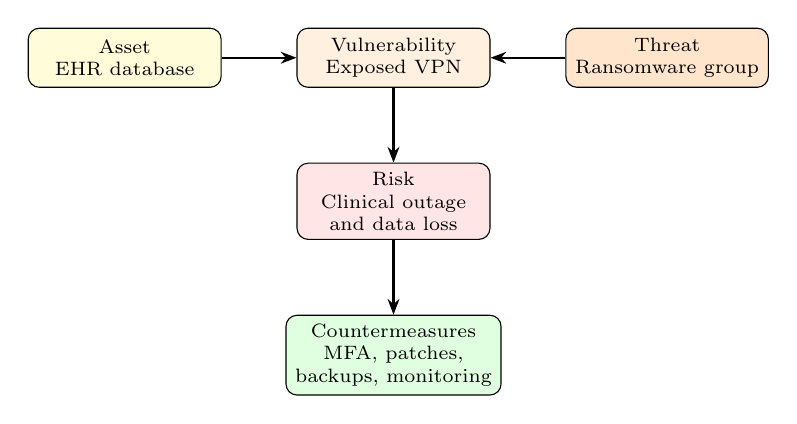
\begin{tikzpicture}[
    node distance=0.95cm,
    box/.style={draw, rounded corners, align=center, minimum width=2.45cm, minimum height=0.75cm, font=\scriptsize},
    risk/.style={box, fill=red!10},
    link/.style={-{Stealth[length=2mm]}, thick}
]
\node[box, fill=yellow!15] (asset) {Asset\\EHR database};
\node[box, right=of asset, fill=orange!12] (vuln) {Vulnerability\\Exposed VPN};
\node[box, right=of vuln, fill=orange!20] (threat) {Threat\\Ransomware group};
\node[risk, below=of vuln] (risk) {Risk\\Clinical outage\\and data loss};
\node[box, below=of risk, fill=green!12] (control) {Countermeasures\\MFA, patches,\\backups, monitoring};
\draw[link] (asset) -- (vuln);
\draw[link] (threat) -- (vuln);
\draw[link] (vuln) -- (risk);
\draw[link] (risk) -- (control);
\end{tikzpicture}
\end{center}

\begin{block}{Reading the scheme}
Risk emerges when a valuable hospital asset is reachable through an exploitable weakness.
\end{block}
\end{frame}

\begin{frame}[c]{Risk Matrix}
\begin{block}{Concept}
A risk matrix compares \textbf{likelihood} and \textbf{impact}. It is a communication tool, not a
mathematical proof.
\end{block}

\begin{exampleblock}{Hospital example}
A rare failure in a public display screen may be low priority. A likely phishing campaign against
nurses with access to medication orders deserves immediate attention.
\end{exampleblock}
\end{frame}

\begin{frame}[c]{Estimating Likelihood}
\begin{block}{Concept}
\textbf{Likelihood} is an informed judgement about how plausible an event is in a defined time
period. It should combine evidence about the threat, the weakness, and the hospital environment.
\end{block}

\begin{itemize}
    \item \textbf{Threat activity}: are attackers currently exploiting this kind of target?
    \item \textbf{Exposure}: is the vulnerable system reachable from the Internet, VPN, Wi-Fi, or vendors?
    \item \textbf{Control strength}: are MFA, patches, monitoring, and segmentation effective?
    \item \textbf{History}: has the hospital or a peer organisation seen similar incidents?
\end{itemize}
\end{frame}

\begin{frame}[c]{Likelihood in the Hospital}
\begin{exampleblock}{Hospital example}
For St. Isidore, phishing against staff is \textbf{high likelihood}: it is common, cheap, and targets
busy users. Theft of a server from the data centre is \textbf{low likelihood}: physical access is
restricted and monitored.
\end{exampleblock}

\begin{block}{Practical rule}
Do not estimate likelihood from intuition alone. Use logs, vulnerability scans, incident history,
threat intelligence, audit findings, and knowledge of clinical workflows.
\end{block}
\end{frame}

\begin{frame}[c]{Example Risk Matrix}
\begin{center}
\scriptsize
\renewcommand{\arraystretch}{1.35}
\begin{tabular}{>{\bfseries}p{0.18\textwidth} p{0.22\textwidth} p{0.22\textwidth} p{0.22\textwidth}}
\toprule
 & \textbf{Low impact} & \textbf{Moderate impact} & \textbf{High impact} \\
\midrule
\textbf{High likelihood}
& \cellcolor{yellow!35} Phishing email to generic mailbox
& \cellcolor{orange!35} Phishing nurses with portal access
& \cellcolor{red!35} Exploited VPN reaching clinical systems \\
\textbf{Medium likelihood}
& \cellcolor{green!25} Public screen misconfiguration
& \cellcolor{yellow!35} Appointment system outage
& \cellcolor{orange!35} Malware on ward workstation \\
\textbf{Low likelihood}
& \cellcolor{green!15} Cafeteria page defacement
& \cellcolor{green!25} Theft of encrypted laptop
& \cellcolor{yellow!35} Data-centre fire with tested failover \\
\bottomrule
\end{tabular}
\end{center}

\begin{block}{Reading the matrix}
Items in red or orange are discussed first. Green items are not ignored, but they usually receive
lighter controls or later treatment.
\end{block}
\end{frame}

\begin{frame}[c]{Residual Risk}
\begin{block}{Concept}
\textbf{Residual risk} is the risk that remains after countermeasures are applied.
\end{block}

\begin{exampleblock}{Hospital example}
MFA reduces account takeover, but a tired doctor may still approve a fraudulent push request.
Training, number matching, monitoring, and help-desk procedures reduce the remaining risk.
\end{exampleblock}
\end{frame}

\begin{frame}[c]{Recap: Impact and Risk}
\begin{block}{Takeaways}
\begin{itemize}
    \item Impact levels help separate minor inconvenience from patient-safety risk.
    \item Risk combines \textbf{asset value}, \textbf{threats}, \textbf{vulnerabilities}, likelihood, and impact.
    \item A risk matrix helps prioritise, but it does not remove uncertainty.
    \item Controls reduce risk; they rarely remove it completely.
\end{itemize}
\end{block}

\begin{exampleblock}{Hospital checkpoint}
The same ransomware threat is more urgent when it can reach the EHR, lab, and pharmacy systems
than when it can only affect an isolated public kiosk.
\end{exampleblock}
\end{frame}

\section{Vulnerabilities and Attacks}
\sectiontitleframe{Vulnerabilities and Attacks}

\begin{frame}[c]{Section Context: Vulnerabilities and Attacks}
\begin{block}{What we are talking about}
This section explains how security failures start. A vulnerability is the weakness; an attack is
the attempt to exploit it; the attacker may be inside or outside the organisation.
\end{block}

\begin{exampleblock}{Hospital lens}
At St. Isidore, the same patient record can be threatened by a stolen password, a curious employee,
an exposed server, or a malware-infected workstation. The defence depends on the attack path.
\end{exampleblock}
\end{frame}

\begin{frame}[c]{Vulnerability Categories}
\begin{block}{Concept}
Vulnerabilities can be grouped by the security property they endanger.
\end{block}

\begin{itemize}
    \item \textbf{Corrupted}: integrity is lost.
    \item \textbf{Leaky}: confidentiality is lost.
    \item \textbf{Unavailable}: availability is lost.
\end{itemize}

\begin{exampleblock}{Hospital example}
A wrong lab value is \textit{corrupted}; a public folder with patient PDFs is \textit{leaky}; a locked
ransomware database is \textit{unavailable}.
\end{exampleblock}
\end{frame}

\begin{frame}[c]{Active Attacks}
\begin{block}{Concept}
An \textbf{active attack} alters resources or influences system behaviour.
\end{block}

\begin{exampleblock}{Hospital example}
An attacker changes a discharge summary, modifies DNS settings, installs malware on a nurse
workstation, or floods a patient portal until it stops responding.
\end{exampleblock}
\end{frame}

\begin{frame}[c]{Passive Attacks}
\begin{block}{Concept}
A \textbf{passive attack} observes or collects information without directly changing the system.
\end{block}

\begin{exampleblock}{Hospital example}
Someone connected to an insecure guest Wi-Fi captures unencrypted traffic and learns which
devices communicate with the radiology system.
\end{exampleblock}
\end{frame}

\begin{frame}[c]{Insider Attacks}
\begin{block}{Concept}
An \textbf{insider attack} is performed by someone who already has authorised access but uses it
in an unauthorised way.
\end{block}

\begin{exampleblock}{Hospital example}
A staff member opens the record of a neighbour without a care-related reason. The account is
valid; the use is not.
\end{exampleblock}
\end{frame}

\begin{frame}[c]{Outsider Attacks}
\begin{block}{Concept}
An \textbf{outsider attack} comes from outside the security perimeter: criminals, opportunistic
attackers, hostile actors, or compromised third parties.
\end{block}

\begin{exampleblock}{Hospital example}
A criminal group sends phishing emails to hospital staff to steal credentials and access the EHR
remotely.
\end{exampleblock}
\end{frame}

\begin{frame}[c]{Preventive Countermeasures}
\begin{block}{Concept}
\textbf{Preventive controls} try to stop an attack before it succeeds.
\end{block}

\begin{exampleblock}{Hospital example}
St. Isidore uses MFA for remote access, network segmentation between guest Wi-Fi and clinical
systems, endpoint protection, patched servers, and role-based access control.
\end{exampleblock}
\end{frame}

\begin{frame}[c]{Detect and Recover}
\begin{block}{Concept}
\textbf{Detect-and-recover controls} assume that prevention can fail. They identify attacks,
contain damage, and restore trustworthy service.
\end{block}

\begin{exampleblock}{Hospital example}
The security team monitors unusual EHR access, isolates infected laptops, restores clean backups,
and reviews logs after an incident.
\end{exampleblock}
\end{frame}

\begin{frame}[c]{Recap: Vulnerabilities and Attacks}
\begin{block}{Takeaways}
\begin{itemize}
    \item Vulnerabilities can make systems \textbf{corrupted}, \textbf{leaky}, or \textbf{unavailable}.
    \item Active attacks change systems; passive attacks observe them.
    \item Insider attacks misuse legitimate access; outsider attacks cross the perimeter.
    \item Prevention matters, but detection and recovery are essential when prevention fails.
\end{itemize}
\end{block}

\begin{exampleblock}{Hospital checkpoint}
An exposed VPN, a stolen account, and weak backup protection are different weaknesses, but
together they can form one ransomware path.
\end{exampleblock}
\end{frame}

\section{Threat Classes}
\sectiontitleframe{Threat Classes}

\begin{frame}[c]{Section Context: Threat Classes}
\begin{block}{What we are talking about}
This section classifies common threat patterns. Instead of memorising isolated attack names, we
connect each threat to the security property it damages: confidentiality, integrity, availability,
or control of resources.
\end{block}

\begin{exampleblock}{Hospital lens}
The hospital scenario helps distinguish \textit{leaking a record}, \textit{changing a record},
\textit{blocking a service}, and \textit{taking over a system}. Each failure calls for different
controls and response procedures.
\end{exampleblock}
\end{frame}

\begin{frame}[c]{Unauthorised Disclosure}
\begin{block}{Concept}
\textbf{Unauthorised disclosure} is a confidentiality threat: information reaches an entity that
should not receive it.
\end{block}

\begin{exampleblock}{Hospital example}
A misconfigured cloud storage bucket exposes discharge letters containing patient names,
diagnoses, and medication lists.
\end{exampleblock}
\end{frame}

\begin{frame}[c]{Exposure}
\begin{block}{Concept}
\textbf{Exposure} can be intentional or accidental. It occurs when sensitive information is made
visible to the wrong audience.
\end{block}

\begin{exampleblock}{Hospital example}
A spreadsheet of HIV clinic appointments is emailed to a public mailing list by mistake.
\end{exampleblock}
\end{frame}

\begin{frame}[c]{Interception}
\begin{block}{Concept}
\textbf{Interception} occurs when communication is observed in transit.
\end{block}

\begin{exampleblock}{Hospital example}
An attacker captures unencrypted traffic between an old bedside device and a monitoring server.
\end{exampleblock}
\end{frame}

\begin{frame}[c]{Inference}
\begin{block}{Concept}
\textbf{Inference} means deriving sensitive information from indirect signals, partial data, or
metadata.
\end{block}

\begin{exampleblock}{Hospital example}
Even if message contents are encrypted, repeated traffic from oncology to a patient's room at
specific times may reveal sensitive clinical context.
\end{exampleblock}
\end{frame}

\begin{frame}[c]{Intrusion}
\begin{block}{Concept}
\textbf{Intrusion} is unauthorised access that bypasses controls and reaches protected resources.
\end{block}

\begin{exampleblock}{Hospital example}
An attacker exploits a vulnerable patient portal and downloads appointment histories from the
backend database.
\end{exampleblock}
\end{frame}

\begin{frame}[c]{Masquerade}
\begin{block}{Concept}
\textbf{Masquerade} is impersonation: one entity pretends to be another.
\end{block}

\begin{exampleblock}{Hospital example}
A stolen nurse account is used to open patient records. To the EHR, the request looks like it
came from the nurse unless stronger authentication and anomaly detection intervene.
\end{exampleblock}
\end{frame}

\begin{frame}[c]{Falsification}
\begin{block}{Concept}
\textbf{Falsification} replaces valid information with false information.
\end{block}

\begin{exampleblock}{Hospital example}
Changing a blood type, medication dose, or lab result can directly influence clinical decisions.
Integrity failures can therefore become safety incidents.
\end{exampleblock}
\end{frame}

\begin{frame}[c]{Repudiation}
\begin{block}{Concept}
\textbf{Repudiation} occurs when someone denies an action, such as sending, approving, or receiving
data.
\end{block}

\begin{exampleblock}{Hospital example}
A physician denies approving a high-risk medication order. Strong authentication, audit logs, and
timestamps help reconstruct what happened.
\end{exampleblock}
\end{frame}

\begin{frame}[c]{Disruption}
\begin{block}{Concept}
\textbf{Disruption} threatens availability by preventing normal service.
\end{block}

\begin{exampleblock}{Hospital example}
A denial-of-service attack makes the patient portal unreachable during vaccination booking. Care
continues, but administrative pressure rises quickly.
\end{exampleblock}
\end{frame}

\begin{frame}[c]{Incapacitation}
\begin{block}{Concept}
\textbf{Incapacitation} disables a system or component through physical damage, malware, or severe
failure.
\end{block}

\begin{exampleblock}{Hospital example}
Ransomware encrypts the file server used by radiology. Images cannot be retrieved until recovery
procedures start.
\end{exampleblock}
\end{frame}

\begin{frame}[c]{Obstruction}
\begin{block}{Concept}
\textbf{Obstruction} interferes with communication or overloads resources.
\end{block}

\begin{exampleblock}{Hospital example}
An attacker floods the VPN gateway. Doctors working from home cannot connect to review urgent
test results.
\end{exampleblock}
\end{frame}

\begin{frame}[c]{Usurpation}
\begin{block}{Concept}
\textbf{Usurpation} occurs when an unauthorised entity takes control of a logical or physical
resource.
\end{block}

\begin{exampleblock}{Hospital example}
Compromised hospital workstations become part of a botnet and are used to attack another
organisation, damaging both security and reputation.
\end{exampleblock}
\end{frame}

\begin{frame}[c]{Recap: Threat Classes}
\begin{block}{Takeaways}
\begin{itemize}
    \item \textbf{Disclosure} attacks expose information through exposure, interception, inference, or intrusion.
    \item \textbf{Deception} attacks undermine trust through masquerade, falsification, or repudiation.
    \item \textbf{Disruption} attacks reduce availability through incapacity or obstruction.
    \item \textbf{Usurpation} means unauthorised control of hospital resources.
\end{itemize}
\end{block}

\begin{exampleblock}{Hospital checkpoint}
If a forged lab message is accepted by the EHR, the problem is not only technical: it can affect
diagnosis, treatment, auditability, and patient safety.
\end{exampleblock}
\end{frame}

\section{Attack Surface}
\sectiontitleframe{Attack Surface}

\begin{frame}[c]{Section Context: Attack Surface}
\begin{block}{What we are talking about}
This section brings the lesson together by asking where an attacker can touch the hospital
environment. Attack surface analysis maps entry points, weaknesses, paths, controls, and assets.
\end{block}

\begin{exampleblock}{Hospital lens}
For St. Isidore, the attack surface includes technology and people: VPN, email, patient portal,
medical devices, vendor access, APIs, Wi-Fi, cloud systems, and staff workflows.
\end{exampleblock}
\end{frame}

\begin{frame}[c]{Attack Surface}
\begin{block}{Concept}
The \textbf{attack surface} is the set of points where an attacker can interact with, influence, or
observe a system.
\end{block}

\begin{exampleblock}{Hospital example}
The patient portal, VPN, Wi-Fi, email, medical devices, vendor support accounts, APIs, and staff
workstations are all part of the hospital attack surface.
\end{exampleblock}
\end{frame}

\begin{frame}[c]{Network Attack Surface}
\begin{block}{Concept}
The network attack surface includes exposed ports, services, protocols, remote access paths, and
network boundaries.
\end{block}

\begin{exampleblock}{Hospital example}
An old remote administration service left open on a radiology server creates a direct path into a
clinical network segment.
\end{exampleblock}
\end{frame}

\begin{frame}[c]{Software Attack Surface}
\begin{block}{Concept}
The software attack surface includes input channels, APIs, file uploads, web forms, parsers,
legacy components, and configuration interfaces.
\end{block}

\begin{exampleblock}{Hospital example}
A patient portal upload feature accepts PDF documents. If parsing is vulnerable, a malicious file
may compromise the server.
\end{exampleblock}
\end{frame}

\begin{frame}[c]{Human Attack Surface}
\begin{block}{Concept}
The human attack surface includes phishing, social engineering, unclear procedures, fatigue, and
pressure during urgent work.
\end{block}

\begin{exampleblock}{Hospital example}
A caller pretending to be from IT asks a nurse to approve an MFA prompt. Training and clear
help-desk procedures reduce this path.
\end{exampleblock}
\end{frame}

\begin{frame}[c]{Analysing Attack Paths}
\begin{block}{Concept}
Attack surface analysis maps entry points, vulnerabilities, controls, and assets that could be
reached.
\end{block}

\begin{exampleblock}{Hospital example}
Phishing email $\rightarrow$ stolen credentials $\rightarrow$ VPN access $\rightarrow$ file share
$\rightarrow$ ransomware. Controls can interrupt the path at several points.
\end{exampleblock}
\end{frame}

\begin{frame}[c]{Scheme: Example Attack Path}
\begin{center}
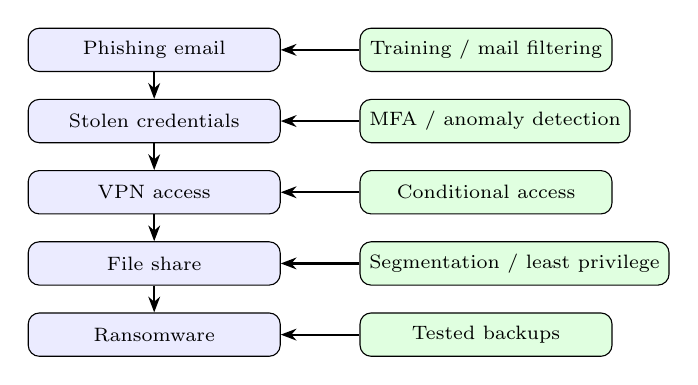
\begin{tikzpicture}[
    node distance=0.34cm,
    attackstep/.style={draw, rounded corners, align=center, minimum width=3.2cm, minimum height=0.55cm, font=\scriptsize, fill=blue!8},
    stop/.style={draw, rounded corners, align=center, minimum width=3.2cm, minimum height=0.55cm, font=\scriptsize, fill=green!12},
    link/.style={-{Stealth[length=2mm]}, thick}
]
\node[attackstep] (phish) {Phishing email};
\node[stop, right=1.0cm of phish] (train) {Training / mail filtering};
\node[attackstep, below=of phish] (cred) {Stolen credentials};
\node[stop, right=1.0cm of cred] (mfa) {MFA / anomaly detection};
\node[attackstep, below=of cred] (vpn) {VPN access};
\node[stop, right=1.0cm of vpn] (access) {Conditional access};
\node[attackstep, below=of vpn] (share) {File share};
\node[stop, right=1.0cm of share] (seg) {Segmentation / least privilege};
\node[attackstep, below=of share] (ransom) {Ransomware};
\node[stop, right=1.0cm of ransom] (backup) {Tested backups};
\draw[link] (phish) -- (cred);
\draw[link] (cred) -- (vpn);
\draw[link] (vpn) -- (share);
\draw[link] (share) -- (ransom);
\draw[link] (train) -- (phish);
\draw[link] (mfa) -- (cred);
\draw[link] (access) -- (vpn);
\draw[link] (seg) -- (share);
\draw[link] (backup) -- (ransom);
\end{tikzpicture}
\end{center}

\begin{block}{Takeaway}
Controls are stronger when they interrupt the path before attackers reach clinical assets.
\end{block}
\end{frame}

\begin{frame}[c]{Reducing Attack Surface}
\begin{block}{Concept}
Reducing attack surface means removing unnecessary exposure and strengthening unavoidable
exposure.
\end{block}

\begin{exampleblock}{Hospital example}
St. Isidore closes unused ports, removes stale accounts, segments medical devices, limits vendor
access windows, and monitors remote access.
\end{exampleblock}
\end{frame}

\begin{frame}[c]{Recap: Attack Surface}
\begin{block}{Takeaways}
\begin{itemize}
    \item Attack surface is the set of places an attacker can interact with or observe a system.
    \item Network, software, and human surfaces often connect into one attack path.
    \item Reducing exposure is as important as strengthening unavoidable exposure.
    \item Attack-path thinking helps place controls before attackers reach clinical assets.
\end{itemize}
\end{block}

\begin{exampleblock}{Hospital checkpoint}
Phishing $\rightarrow$ stolen credentials $\rightarrow$ VPN $\rightarrow$ file share
$\rightarrow$ ransomware is a path. MFA, segmentation, least privilege, monitoring, and backups
interrupt it at different points.
\end{exampleblock}
\end{frame}

\section{Design and Policy}
\sectiontitleframe{Design and Policy}

\begin{frame}[c]{Section Context: Design and Policy}
\begin{block}{What we are talking about}
This section shifts from attacks to design choices. Secure systems are not created only by adding
tools; they are shaped by principles, policies, workflows, and evidence that controls actually work.
\end{block}

\begin{exampleblock}{Hospital lens}
St. Isidore must design access rules, emergency override, remote access, logging, backup, and
incident response so that security supports care instead of fighting it.
\end{exampleblock}
\end{frame}

\begin{frame}[c]{Secure Design Principles}
\begin{block}{Concept}
Classic secure design principles reduce complexity, minimise trust, and make failures safer
\cite{saltzer_schroeder_1975}.
\end{block}

\begin{exampleblock}{Hospital example}
St. Isidore applies these principles when designing EHR access, emergency override, remote access,
network segmentation, audit logging, and backup recovery.
\end{exampleblock}
\end{frame}

\begin{frame}[c]{Economy of Mechanism}
\begin{block}{Principle}
Security mechanisms should be as simple as possible, so they can be understood, implemented, and
verified.
\end{block}

\begin{exampleblock}{Hospital example}
A simple role model for nurse, physician, pharmacist, and administrator is easier to review than
hundreds of undocumented special permissions.
\end{exampleblock}
\end{frame}

\begin{frame}[c]{Fail-Safe Defaults}
\begin{block}{Principle}
Access should be denied unless permission is explicitly granted.
\end{block}

\begin{exampleblock}{Hospital example}
New temporary staff accounts should start with no EHR access. Access is added only after role,
department, and supervisor approval are confirmed.
\end{exampleblock}
\end{frame}

\begin{frame}[c]{Complete Mediation}
\begin{block}{Principle}
Every access should be checked, not only the first one.
\end{block}

\begin{exampleblock}{Hospital example}
If a doctor changes department, the EHR should re-check access rights on each record request,
not rely on permissions cached months earlier.
\end{exampleblock}
\end{frame}

\begin{frame}[c]{Open Design}
\begin{block}{Principle}
Security should not depend on keeping the mechanism secret. Secrets should be limited to keys,
passwords, and credentials.
\end{block}

\begin{exampleblock}{Hospital example}
The hospital should use well-reviewed encryption protocols rather than a custom ``secret''
algorithm for transmitting lab results.
\end{exampleblock}
\end{frame}

\begin{frame}[c]{Least Privilege}
\begin{block}{Principle}
Users, services, and devices should receive only the permissions needed for their tasks.
\end{block}

\begin{exampleblock}{Hospital example}
A kiosk used for patient check-in should not have permission to browse the full EHR database.
If compromised, its limited role reduces damage.
\end{exampleblock}
\end{frame}

\begin{frame}[c]{Separation of Privilege}
\begin{block}{Principle}
Critical actions should require more than one condition, role, or approval.
\end{block}

\begin{exampleblock}{Hospital example}
Changing a patient's identity record may require both administrative approval and a separate
verification by the medical records office.
\end{exampleblock}
\end{frame}

\begin{frame}[c]{Layering and Defence in Depth}
\begin{block}{Principle}
\textbf{Layering} means using multiple overlapping controls, so one failure does not expose the
whole system.
\end{block}

\begin{exampleblock}{Hospital example}
Remote access uses VPN, MFA, device compliance checks, network segmentation, EHR role checks,
and logging. Each layer limits what happens if another layer fails.
\end{exampleblock}
\end{frame}

\begin{frame}[c]{Scheme: Defence in Depth}
\begin{center}
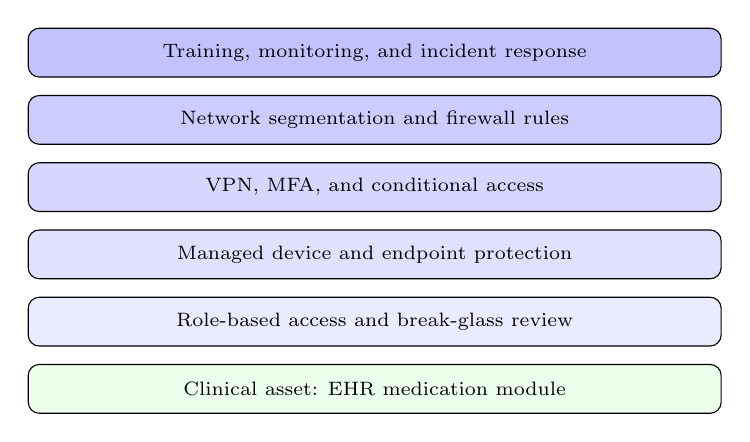
\begin{tikzpicture}[
    layer/.style={draw, rounded corners, align=center, minimum width=8.8cm, minimum height=0.62cm, font=\scriptsize},
    node distance=0.22cm
]
\node[layer, fill=green!8] (ehr) {Clinical asset: EHR medication module};
\node[layer, above=of ehr, fill=blue!8] (rbac) {Role-based access and break-glass review};
\node[layer, above=of rbac, fill=blue!12] (device) {Managed device and endpoint protection};
\node[layer, above=of device, fill=blue!16] (mfa) {VPN, MFA, and conditional access};
\node[layer, above=of mfa, fill=blue!20] (seg) {Network segmentation and firewall rules};
\node[layer, above=of seg, fill=blue!24] (train) {Training, monitoring, and incident response};
\end{tikzpicture}
\end{center}

\begin{block}{Reading the scheme}
No single layer is trusted to be perfect. Each layer reduces what an attacker can do next.
\end{block}
\end{frame}

\begin{frame}[c]{Psychological Acceptability}
\begin{block}{Principle}
Security controls should be understandable and usable enough that people can follow them during
real work.
\end{block}

\begin{exampleblock}{Hospital example}
If login takes too long during ward rounds, staff may share accounts. A better design protects
security while respecting clinical pace.
\end{exampleblock}
\end{frame}

\begin{frame}[c]{Security Policy}
\begin{block}{Concept}
A security policy turns security goals into organisational rules: who may access what, under
which conditions, with what logging and responsibilities.
\end{block}

\begin{exampleblock}{Hospital example}
The policy states that staff may access records only for care, operations, payment, or approved
research. Curiosity access is prohibited even if the account technically works.
\end{exampleblock}
\end{frame}

\begin{frame}[c]{Security Trade-Offs}
\begin{block}{Concept}
Security must balance protection, usability, cost, performance, legal duties, and patient care.
\end{block}

\begin{exampleblock}{Hospital example}
Strict session timeouts protect unattended workstations, but overly aggressive timeouts may delay
care. The hospital may use badge tap-in, short idle locks, and fast re-authentication.
\end{exampleblock}
\end{frame}

\begin{frame}[c]{Prevention}
\begin{block}{Concept}
\textbf{Prevention} aims to stop attacks before they succeed.
\end{block}

\begin{exampleblock}{Hospital example}
Patch management, MFA, network segmentation, secure configuration, and phishing-resistant
authentication reduce the chance of compromise.
\end{exampleblock}
\end{frame}

\begin{frame}[c]{Detection}
\begin{block}{Concept}
\textbf{Detection} identifies suspicious activity, misuse, policy violations, or confirmed
intrusions.
\end{block}

\begin{exampleblock}{Hospital example}
An alert triggers when one account opens hundreds of patient records across unrelated wards in
ten minutes.
\end{exampleblock}
\end{frame}

\begin{frame}[c]{Response}
\begin{block}{Concept}
\textbf{Response} contains an incident, limits further damage, preserves evidence, and coordinates
communication.
\end{block}

\begin{exampleblock}{Hospital example}
When malware is detected, IT isolates the workstation, disables the account, informs clinical
leadership, and checks whether patient care is affected.
\end{exampleblock}
\end{frame}

\begin{frame}[c]{Recovery}
\begin{block}{Concept}
\textbf{Recovery} restores services and data to a trustworthy state after an incident.
\end{block}

\begin{exampleblock}{Hospital example}
After ransomware, the hospital rebuilds servers from clean images, restores tested backups, and
reconciles paper medication orders entered during downtime.
\end{exampleblock}
\end{frame}

\begin{frame}[c]{Assurance}
\begin{block}{Concept}
\textbf{Assurance} is confidence that security measures satisfy their requirements.
\end{block}

\begin{exampleblock}{Hospital example}
The hospital does not merely assume backups work. It performs restoration tests and records the
time needed to recover critical systems.
\end{exampleblock}
\end{frame}

\begin{frame}[c]{Evaluation}
\begin{block}{Concept}
\textbf{Evaluation} checks a system against defined criteria through testing, review, audit,
certification, or formal analysis.
\end{block}

\begin{exampleblock}{Hospital example}
Before buying a new telemedicine platform, St. Isidore reviews encryption, logging, access
control, data retention, vendor support, and incident notification terms.
\end{exampleblock}
\end{frame}

\begin{frame}[c]{Recap: Design and Policy}
\begin{block}{Takeaways}
\begin{itemize}
    \item Design principles reduce complexity and limit damage when something fails.
    \item Policy translates security goals into organisational rules and responsibilities.
    \item Security is a trade-off among protection, usability, cost, performance, and care delivery.
    \item Prevention, detection, response, recovery, assurance, and evaluation form a lifecycle.
\end{itemize}
\end{block}

\begin{exampleblock}{Hospital checkpoint}
An emergency-access feature is acceptable only if it is fast enough for care, limited in scope,
logged, reviewed, and tested.
\end{exampleblock}
\end{frame}


\begin{frame}[c]{Connecting the Concepts}
\begin{block}{The full picture}
Security starts with objectives, but it becomes practical only when those objectives are connected
to systems, risks, attacks, exposure, and design choices.
\end{block}

\begin{exampleblock}{St. Isidore Hospital}
A stolen credential is not only an \textit{access management} issue. It can expose patient data,
change clinical records, interrupt services, trigger GDPR obligations, and reveal weaknesses in
network design, monitoring, and recovery.
\end{exampleblock}
\end{frame}

\begin{frame}[c]{Bridge to Later Lessons}
\begin{block}{What comes next}
Later lessons will turn today's vocabulary into concrete controls.
\end{block}

\begin{itemize}
    \item \textbf{Networking}: where hospital systems connect, and where segmentation helps.
    \item \textbf{Access management}: how users, roles, MFA, and break-glass access are governed.
    \item \textbf{Encryption}: how data is protected at rest, in transit, and through key management.
    \item \textbf{GDPR}: how privacy, security, accountability, and breach response become legal duties.
\end{itemize}
\end{frame}

\begin{frame}[c]{Doubts? Mail me!}
\begin{center}
\Large g.pisano@unibo.it
\end{center}
\end{frame}

\begin{frame}[allowframebreaks]
\titlepage
\end{frame}

%===============================================================================
\section*{\refname}
%===============================================================================

\setbeamertemplate{page number in head/foot}{}
%/////////
\begin{frame}[c,allowframebreaks,noframenumbering]{\refname}
%\begin{frame}[t,allowframebreaks,noframenumbering]{\refname}
%	\tiny
	\scriptsize
%	\footnotesize
	\bibliographystyle{apalike-AMS}
	\bibliography{main}
\end{frame}

\end{document}
